\section{Introduction}
\label{sec:intro}
Scaling laws have established that model performance improves predictably with increased FLOPs \citep{kaplan2020scalinglawsneurallanguage, hoffmann2022trainingcomputeoptimallargelanguage}, typically by increasing parameter count or training data.
These scaling laws suggest that FLOP-optimal training increases parameters and training data in tandem following empirical power laws.
As a result, the depth and width of state-of-the-art models have grown in an effort to scale with data, subsequently inflating the memory footprint to deploy these models \citep{dettmers2023case4bitprecisionkbit, lin2024awqactivationawareweightquantization}.


However, as inference deployments take on an increasingly large portion of compute \citep{touvron2023llamaopenefficientfoundation}, and deployments begin to move to the edge \citep{moon2024lpulatencyoptimizedhighlyscalable, narayan2025minionscostefficientcollaborationondevice}, there is increasing interest in scaling model quality without increasing parameters.
One mechanism to do this is layer-looped models, such as looped transformers \citep{dehghaniUniversalTransformers2019, geiping_scaling_2025, zhuScalingLatentReasoning2025}, which iteratively loop activations through a block of layers.
Initial results have been encouraging, with looped models matching the quality of larger fixed-depth architectures~\citep{geiping_scaling_2025, zhuScalingLatentReasoning2025}. Moreover, they show potential for latent reasoning~\citep{avi_learn_algorithm, yangLoopedTransformersAre2023} and per-token adaptive compute \citep{geiping_scaling_2025,mcleish_retrofitted_recurrence}.


\begin{figure*}[t]
    \centering
    \vspace{-0.3em}
    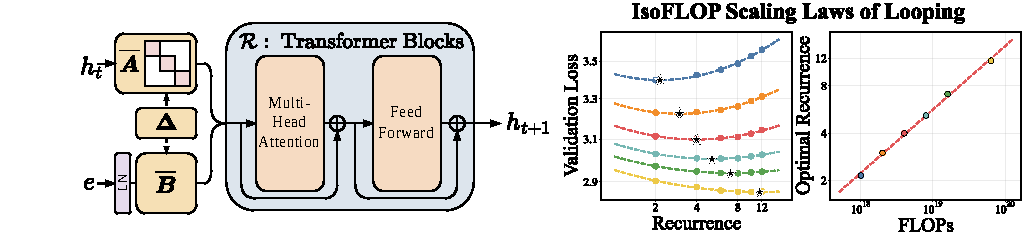
\includegraphics[trim={1.36cm 0 0 0cm},clip, width=\linewidth]{figures/main/main_fig.pdf}
    \vspace{-1.6em}
    \caption{\textbf{\sysname and the Scaling Laws of Looping.}
    (\emph{Left}) \sysname constrains the spectral norm of $\dA$ and normalizes the input injection, stabilizing the residual stream $h_t$ across loops. (\emph{Right}) We observe looping to be an orthogonal axis of scaling compute which follows a power law.}
    \label{fig:block-diagram}
    \vspace{-1em}
\end{figure*}

Unfortunately, prior research \citep{geiping_scaling_2025, mcleish_retrofitted_recurrence, LoopFormerElasticDepthLooped2025} and our work observe these models' training to be unstable, exhibiting residual state explosion and loss spikes.
Since these models loop the layers of complex non-linear architectures (e.g., transformer blocks \citep{vaswani2023attentionneed}), the source of instability in looped models can be difficult to understand analytically.
As a result, training requires sensitive hyperparameter selection and {residual normalization} (e.g., Post-Norm) to correct this instability \citep{geiping_scaling_2025}. 
Furthermore, even in convergent training runs, we observe loss spikes as looped models train on stochastic amounts of depth to induce stronger test-time scaling \citep{anilPathIndependentEquilibrium}.
In this paper, we study this instability and ask whether stabilizing these models can unlock looping as a predictable, orthogonal axis for scaling compute.

To analyze instability, we observe that prior looped architectures can be recast as a nonlinear time-variant dynamical system over the residual stream \citep{olsson2022incontextlearninginductionheads}, taking the form:
\begin{equation}
    \label{eq:alpha-af}
    h_{t+1} = \dA h_t + \dB e + \overline{\mathcal{R}}(h_t, e),
\end{equation}
where for an input $e$, the hidden state $h$ across the depth of an architecture is modulated by $\dA$, controlling the balance between prior and current residual states; $\dB$, conditioning the residual on the input $e$; and a non-linear operator $\overline{\mathcal{R}}$, which subsumes the original transformer modules (e.g., Attention, MLPs).
By linearizing this framework (e.g., removing $\overline{\mathcal{R}}$), we observe that \cref{eq:alpha-af} resolves to a linear time invariant (LTI) system from which classic control theory can be used to infer divergence conditions on the residual stream based on the spectral norm of $\dA$.
We observe that prior looped architectures can learn unstable parameterizations of $\dA$, which we empirically find to induce residual stream explosion (see \cref{fig:spectral-norm}).

To address these issues, we propose \emph{\textbf{\sysname}}, a novel looped transformer that corrects the parameter instability conditions of \cref{eq:alpha-af} and uses algorithmic fixes to reduce loss spikes during training. \emph{\textbf{\sysname}} explicitly uses discretization on a continuous representation $\A$ of \cref{eq:alpha-af} and parametrizes $\A$ as a negative diagonal matrix, constraining the spectral norm to prevent residual explosion in looped layers.
Additionally, \sysname introduces a normalization on $e$, which empirically prevents loss spikes in late stages of training. Finally, \sysname 
modifies the training algorithm (which aims to minimize the expected loss over variable depths) by enabling intra-batch per-sequence depth sampling to further reduce loss spikes.


We evaluate \sysname on end-to-end quality, training FLOP scaling, and test-time scaling:
\begin{itemize}[itemsep=0pt,topsep=0pt,leftmargin=*]
    \item\textbf{End-to-End Quality.} We compare \sysname against parameter- and data-matched RDMs \citep{geiping_scaling_2025} and Transformers. Against RDMs, \sysname reduces val. PPL by 6.3\%. When scaled up to 1.3B parameters and 100B tokens, \sysname outperforms parameter-matched Transformers by up to 2.99 and 1.18 points on Core and Core-Extended \citep{li2025datacomplmsearchgenerationtraining} benchmarks, respectively --- matching Transformers up to twice the size. 
    \item\textbf{Training FLOP Scaling.} To evaluate FLOP training scaling, we study scaling laws for looping in a parameter-matched isoFLOP setting (i.e., whether to scale FLOPs with increased data or looping).
    We find that looping introduces an orthogonal scaling axis, similar to parameters and data.
    Specifically, FLOP-optimal training increases looping and data following empirical power laws (see \cref{fig:block-diagram}~[\emph{right}]). 
    \item\textbf{Test-Time Scaling.} We study looping as a mechanism to scale test-time compute, observing that recurrence follows predictable exponential decay with an irreducible loss. We further combine both test-time and training power laws to create a single unifying scaling law for looping in \sysname models.
\end{itemize}





